\subsection*{a)}
Задан потенциал, с учетом которого мы получаем оператор Гамильтона для нашей задачи:
\begin{equation*}
	U(x) = \left\{\begin{aligned}
		-U_0 \ , \ &|x| \leq a \\
		0 \ , \ &|x| \geq a
	\end{aligned}
	\right.
	\hspace{0.5 cm}
	\Rightarrow
	\hspace{0.5 cm}
	\hat{H} = \left\{\begin{aligned}
		\frac{p^2}{2m} - U_0 \ , \ &|x| \leq a \\
		\frac{p^2}{2m} \ , \ &|x| \geq a	
	\end{aligned}
	\right.
\end{equation*}
Тогда решаем уравнение Шредингера $\hat{H} \psi = E \psi$ вне и снаружи ямы, помня что $\hat{p} = - i \hbar \frac{\partial}{\partial x}$
\begin{equation*}
\frac{- \hbar^2}{2 m} \psi + (\hat{U} - E) = 0
\hspace{0.5 cm}
\Rightarrow
\hspace{0.5 cm}
\left\{\begin{aligned}
	\psi'' + \frac{2 m}{\hbar^2}(U_0 + E) \psi = 0 \\
	\psi'' + \frac{2 m}{\hbar^2} E \psi = 0
\end{aligned}\right.
\end{equation*}
Посмотрим теперь на движение частицы в неглубокой потенциальной яме 
\begin{equation*}
    U(x) = \left\{\begin{aligned}
        - &U_0, |x| < a;
        &0, |x| \geq a.
    \end{aligned}\right.
    \hspace{10 mm} 
    \hat{H} = \frac{\hat{p}^2}{2m} + \hat{U}(x).
\end{equation*}
Так как речь идёт про связанные состояния, то будем считать $E<0$, тогда, для удобства, переобозначим $E \to -E$.
Запишем стационарное уравнение Шредингера, сразу раскрывая $U(r)$, выделяем две области:
\begin{equation*}
    \left\{\begin{aligned}
        \psi'' + k^2 \psi &= 0,  &|x| < a; \\
        \psi'' - \kappa^2 \psi &= 0, &|x| > a;
    \end{aligned}\right.
    \hspace{10 mm} 
    k^2 = \frac{2m}{\hbar^2} (U_0 - E),
    \hspace{5 mm} 
    \kappa^2 = \frac{2m}{\hbar^2} E,
\end{equation*}
В силу симметричности потенциала ($[\hat{I},\, \hat{H}] = 0$), решения могут быть найдены, как собственные функции оператора инверсии, то есть в виде четных и нечетных функций. Тогда сразу можем выделить два решения:
\begin{equation*}
    \psi^+(x) = \left\{\begin{aligned}
         & A \cos(k x), &|x| < a; \\
         & B e^{- \kappa |x|}, &|x|>a;
    \end{aligned}\right.
    \hspace{10 mm}
    \psi^- (x) = 
    \left\{\begin{aligned}
         & A \sin(k x), & |x| < a; \\
        & B \sign(x) e^{- \kappa |x|}, & |x| > a;
    \end{aligned}\right.
\end{equation*}
где сразу воспользовались $L_2$ интегрируемостью $\psi$ и выбросили решение вида $e^{\kappa x}$.




Осталось воспользоваться гладкостью $\psi(x)$, удобнее будет проверить непрерывность логарифмической производной
\begin{equation*}
    (\ln \psi)' = \frac{\psi'}{\psi},
    \hspace{0.5cm} \Rightarrow \hspace{0.5cm}
    \frac{\psi'(a-\varepsilon)}{\psi(a - \varepsilon)} = \frac{\psi'(a+\varepsilon)}{\psi(a+\varepsilon)},
    \hspace{0.5cm} \Rightarrow \hspace{0.5cm}
    \kappa = k \tan(ka),
    \hspace{5 mm}  \Leftrightarrow \hspace{5 mm} 
    |\cos(ka)| = \frac{ka}{k_0 a},
\end{equation*}
где ввели $k_0^2 = \kappa^2 + k^2$. Получили трансцендентное уравнение на уровни энергии, анализ которого удобнее всего произвести графически (рис. \ref{fig:T2}). Ясно, что спектр не просто дискретен, но и ограничен. Четное состояние существует при $k_0 a > 0$, $N$ четных существует при $k_0 a \geq (N-1) \pi$. Важно, что решения существуют только при $\tg k a > 0$.

Аналогично, через логарифмическую производную нахожим условие на уровни энергии нечетных решений.

\begin{figure}[h]
    \centering
    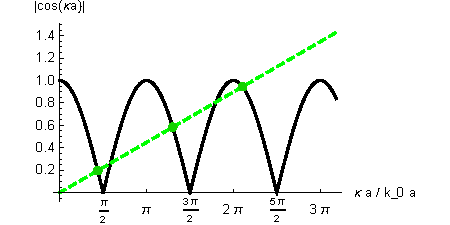
\includegraphics[width=0.4\textwidth]{figures/T2_1.pdf}
    \hspace{5 mm} 
    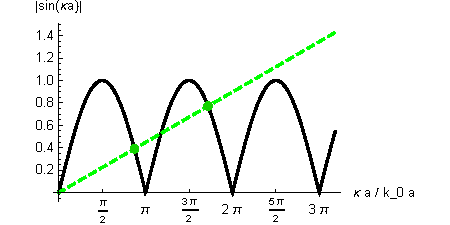
\includegraphics{figures/T2_2.pdf}
    \caption{Трансцендентное уравнение (для четного и нечетного решения) на уровни энергии к задаче Т2}
    \label{fig:T2}
\end{figure}
